%!TEX root = ../Main.tex

\section{Overview of 'Downside Variance Risk Premium'}\label{sec:chapter1}

In 2015,  \textit{ B. Fenou, M.R. Jahan-Parvar and C. Okou} published 'Downside Variance Risk Premium' where they propose a new decomposition of the variance risk premium in terms of upside and downside variance risk premia ($VRP^D$ and $VRP^U$ respectively) and define their difference as skewness risk premium ($SRP$).  Furthermore they evaluate the effectiveness of these measures as equity market returns predictors and find that $VRP^D$ is the main driver of the variance risk premium. 

\vspace{4mm}
The main advantage of this approach is that it relies on two facts that have been proven useful in predicting equity returns: distinguishing between positive and negative returns and including option-implied measures in the analysis. 

\vspace{4mm}
The study is in line with the current asset pricing research that accepts the long term predictability of equity market returns in contrast to the traditional efficient-market hypothesis of market returns unpredictability. 
Furthermore, the paper confirms the results of \textit{ Bollerslev et al. [2009] (henceforth referred to as BTZ)} that suggest the presence of short term equity returns predictors, such as the variance risk premium ($VRP$), defined as the difference between option-implied and realized variance. It is in fact found that the $VRP$ yields superior forecasts for stock market returns over shorter, within-year horizons (typically one quarter ahead). The authors decided to extend this finding and explore the impact of  $VRP^D$ and $VRP^U$ by drawing on the intuition that investors favour good uncertainty over bad uncertainty, as the former increases the potential of substantial gains while the latter increases the likelihood of severe losses.  

\vspace{4mm}
The principal finding of the study is that the $VRP^D$ is the main component of the variance risk premium, making $VRP^U$'s contribution only marginal. Moreover it is found that the skewness risk premia is a priced factor with significant prediction power for aggregate excess returns. In fact, a positive and significant relation is found between the $VRP^D$ and the equity premium, as well as between the skewness risk premia and the equity premium. On average over 80\% of the VRP is compensation for bearing changes in downside risk.  This result is similar to the ones obtained by \textit{Kozhan et al. [2014]}. Hence also the empirical regularities found in the VRP such as the hump-shaped $R^2$ and slope parameter patterns are explained by its downside component.

\vspace{4mm}
The empirical investigation first confirms that skewness, measured as the difference between upside and downside variances, is a priced factor and provides new evidence that the $SRP$, measured as the difference between the risk neutral and historical expectations of skewness, is both priced and has superior predictive power. 
The empirical investigation further highlights the fact that the $SRP$ fills the time gap between the traditional long term predictors of excess returns, such as price-dividend or price-earning ratios, and the short term VRP predictor. There is a contribution of the SRP to the predictability of returns which takes effect beyond the one-quarter-ahead window documented by BTZ. Therefore, the model proposed in the paper closes the horizon gap between short term models such as BTZ and long-horizon predictive models such as \textit{Fama and French [1988], Campbell and Shiller [1988], Cochrane [1991], and Lettau and Ludvigson [2001].}

\vspace{4mm}
Furthermore, it is shown that the prediction power of $VRP^D$ and $SRP$ increases over the term structure of equity returns. This result is robust to the inclusion of a wide variety of common pricing factors, resulting in the independence of the in-sample predictability of aggregate returns by $VRP^D$  and $SRP$ from the other commonly used pricing ratios (eg. price-dividend ratio, price-earning ratio, or default spread). In order to address data-mining concerns, out-of-sample forecasting exercises are conducted to establish that these predictive variables perform at least as well as the other common pricing variables in forecasting excess returns. The out-of-sample forecast ability comparison then confirms that other common predictors do not have a superior forecast ability in comparison with $VRP^D$ and $SRP$.

\vspace{4mm}
The study furthermore tackles the links that macroeconomic announcements and events share with the $VRP^D$ and $SRP$, as seen in \textit{Amengual and Xiu [2014]}. The correlations between $VRP$ components and 124 macroeconomic and financial indicators are documented in a robustness study comparable to \textit{Ludvigson et al. [2009]} and \textit{Feunou et al. [2014]}. A much lower correlation of the considered macroeconomic and financial indicators is found with $VRP^D$ and $SRP$; compared to the one found with the $VRP$, as well as with the $VRP^U$.

\vspace{4mm}
In addition, the study is also relevant to the recent macro-finance literature which emphasizes the importance of higher-order risk attitudes in the determination of equilibrium asset prices. In particular, among these higher-order risk attitudes, we find prudence, which is a precautionary behavior which characterizes the aversion towards downside risk. For example, \textit{Dionne et al. [2014]} show that consumption second-degree expectation dependence risk is a fundamental source of the macroeconomic risk driving asset prices through the use of a standard consumption-based capital asset pricing model . This consumption second-degree expectation dependence risk is a proxy for downside risk, that as already mentioned accounts for nearly 80\% of the equity premium. 

\vspace{4mm}
Finally, the authors \textit{ B. Fenou, M.R. Jahan-Parvar and C. Okou} support theoretically their empirical findings through the construction of an equilibrium consumption-based asset pricing model, where the representative agent is endowed with \textit{Epstein and Zin [1989]} preferences, and where the consumption growth process is affected by distinct upside and downside shocks. It is shown that under common distributional assumptions for shocks to the economy, the equity risk premium, upside and downside variance risk premium and skewness risk premium can be derives in closed form. 

\vspace{4mm}
It is important to notice that the model presented by the authors is not an alternative to jump-tail risk concerns or rare disaster models. The developed framework has as objective to address the asymmetries that are observed in 'normal times', however, it is also well-suited and capable of addressing regularities that emerge from a rare disaster happening, such as the Great Recession of 2007-2009. 


\subsection{Construction of VRP and SRP }
In this section we will briefly report the construction methodology for VRP and SRP used in \textit{Fenou et al. [2015]} .
$VRP^D$ and $SRP$ are two natural and linked components in the framework developed by \textit{B. Fenou, M.R. Jahan-Parvar and C. Okou} and used as short-medium term predictors of the equity market returns. 

\vspace{4mm}
To study the $VRP^D$, nonparametric measures of up and downside realized and risk-neutral semi-variances are constructed by drawing on the vast existing literature of realized and risk-neutral volatility. For this purpose, the downside and upside variance are defined as the realized variance of the negative and positive market returns respectively. It follows that the downside and upside variance risk premium ($VRP^D$ and $VRP^U$) are defined as the difference between option-implied and realized downside and upside variance extracted from high frequency data. As in \textit{Chang, Christoffersen, and Jacobs [2013]}, the construction approach avoids the traditional trade-off problem with estimates of higher moments from historical returns data needing long windows to increase precision but short windows to obtain conditional instead of unconditional estimates. 

\vspace{4mm}
Moreover, a nonparametric measure of skewness is constructed using the difference between upside and downside variances, also called the relative upside variance. The difference between option-implied and realized relative upside variances is then considered a measure of skewness risk premium ($SRP$).
The $SRP$, as already mentioned, is a priced factor hat enhances the predictive power of the $VRP$ to horizons beyond one quarter ahead, filling the gap between the $VRP$ and common long-term equity returns predictors.
 
 \vspace{4mm}
Thus, in order to construct $VRP$ and $SRP$, reliable measures for realized and risk-neutral variance and skewness are needed. The construction of realized downside and upside volatilities (also known as realized semi-variances) is addressed in \textit{Barndorff-Nielsen [2010]} and the consensus in the literature about construction of these measures is followed. Similarly, risk-neutral measures of volatility are constructed following the existing literature such as in the studies of \textit{Carr and Madan [1998, 1999, 2001]}  and\textit{ Bakshi et al.[2003]}. The construction of option-implied downside and upside volatilities is addressed in \textit{Andersen et al. [2014]}.

On the other hand, traditional measures of skewness have well-documented empirical problems \textit{Kim et al [2004]} such as the excessive sensitivity to outliers. These problems are overcome by using alternative and more robust measures such as by using Pearson and Bowley’s skewness measures \textit{Feunou et al. [2013] and Ghysels et al. [2011]} or imposing autoregressive structures to explore time variation in conditional skewness \textit{Harvey and Siddique [1999, 2000]}.


%run: latex, bibtex, latex to get citations.\\
%test citation: \cite{andersen2001}.\\
%Example on how to include graphics and tables, located in the python project.
%For the graphics I created a link to the variance-python/results/graphics file in ``mystyle.tex'' hence only the name of the graphic without .png ending has to be specified.
%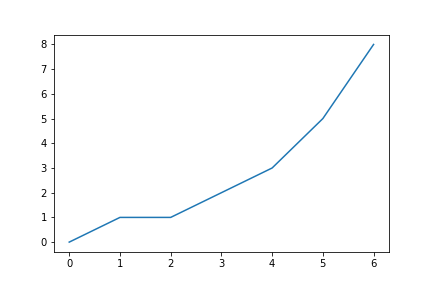
\includegraphics{example_graphic}
%For tables the whole path has to be specified
%\begin{tabular}{lr}
\toprule
{} &  0 \\
\midrule
0 &  0 \\
1 &  1 \\
2 &  1 \\
3 &  2 \\
4 &  3 \\
5 &  5 \\
6 &  8 \\
\bottomrule
\end{tabular}
